\documentclass[14pt,a4paper]{scrartcl}
\usepackage{cmap}
\usepackage[utf8]{inputenc}
\usepackage[T1,T2A]{fontenc}
\usepackage[english,russian]{babel}
\usepackage{relsize}
\usepackage{graphicx}
\usepackage{subfigure}
\usepackage{mathtools}
\usepackage{amssymb}
\usepackage{float}
\usepackage{sidecap}
\usepackage{wrapfig}
\usepackage{caption}
\usepackage[table,xcdraw]{xcolor}
\usepackage{listings}
\usepackage{minted}
\usepackage{multirow}
\usepackage{bigstrut}
\begin{document}
	\begin{titlepage}
	\begin{center}
		\large
		МИНИСТЕРСТВО ОБРАЗОВАНИЯ И НАУКИ\\ РОССИЙСКОЙ ФЕДЕРАЦИИ
		
		\vspace{0.5cm}
		
		МГТУ им Н.Э.Баумана
		\vspace{0.25cm}
		
		Факультет ФН
		
		Кафедра вычислительной математики и математической физики
		\vfill
		
		
		Соколов Арсений Андреевич\\
		\vfill
		
		
		{\LARGE Домашнее задание №5 по математической статистике\\[2mm]
		}
		\bigskip
		
		3 курс, группа ФН11-53Б\\
		Вариант 6
	\end{center}
	\vfill
	
	\newlength{\ML}
	\settowidth{\ML}{«\underline{\hspace{0.7cm}}» \underline{\hspace{2cm}}}
	\hfill\begin{minipage}{0.4\textwidth}
		Преподаватель\\
		\underline{\hspace{3cm}} Т.\,В.~Облакова\\
		«\underline{\hspace{0.7cm}}» \underline{\hspace{1.71cm}} 2019 г.
	\end{minipage}%
	\bigskip
	
	
	\vfill
	
	\begin{center}
		Москва, 2019 г.
	\end{center}
\end{titlepage}

\section*{Задание 1}\label{sec1}
По данной выборке из нормально распределенной генеральной совокупности построить критерий $S_2$ уровня $\alpha = 0.1$ и проверить гипотезу $H_0$: $a=a_0=7.5$  против односторонней альтернативы  $H_2: a>a_0$, если $\sigma$ неизвестно.\\
\textbf{Решение.}\\
Рассмотрим выборку, предложенную нам в условии:
\begin{minted}{R}
> df
[1]  0.653 13.884 11.088  7.409  8.827  5.582  9.747  8.023  8.396
[10]  6.535  6.036  5.251 12.462  9.350  9.770  5.517  6.740 10.759
[19] 10.718  0.840  8.737  2.278  8.447  2.267  8.656  9.460  9.385
[28]  7.924  9.215 10.360  7.239  8.399  7.962  6.712  5.626  7.737
[37]  9.671 13.497 10.708  6.189 10.516  8.845 10.926  8.755  7.728
[46] 12.783  5.300  9.802  5.133  8.534  5.855  5.777 10.128 10.662
[55]  8.307  5.644 10.632  6.060  6.989  5.183  9.587  7.891 15.015
[64]  8.106  9.898 10.504  8.307 10.680  6.788  9.904  6.918  4.250
[73]  8.908  9.837  5.805  6.018  7.735  8.206  5.502  8.473  4.870
[82] 10.159  6.639  7.936  8.149 10.462 12.296  3.403 10.631  7.802
[91]  5.580  8.325 10.687  9.843  9.509  5.668  8.511  8.657  8.835
[100]  9.484
\end{minted}

Предположим, что $H_0$ верна и выберем в качестве статистики:
\begin{equation*}
	t = \frac{\bar{x} - a_0}{s} \sqrt{n},
\end{equation*}
где $\bar{x}$ -- выборочное среднее,\\
a $\; n$ -- объем выборки.\\
Статистика $t$ имеет $t$-распределение с $n-1$ степенями свободы. Соответственно, критическая область для проверки гипотезы $H_0: a = a_0$ против односторонней альтернативы $H_2: a > a_0$ будет состоять из одного полуинтервала $[t_{n-1,1-\alpha};+\infty]$, где $t_{n-1,1-\alpha}$ обозначает квантиль $t-$распределения с $n-1$ степенью свободы и уровня значимости $1-\alpha$.


Рассчитаем нашу статистику:
\begin{minted}{R}
> df_mean <- mean(df)
> df_sd <- sd(df)
> df_len <- length(df)
> df_mean
[1] 8.17393
> df_sd
[1] 2.577009
> df_len
[1] 100
> t_stat <- (mean(df) - a0)/(sd(df)) * sqrt(df_len)
> t_stat
[1] 2.615164
\end{minted}

Это значение должно быть сравнено с $10\%$-ным односторонним критическим пределом, равным $t_{99,0.9}=1.290161$.\\ Выборочное значение статистики выходит за этот предел, следовательно, с уровнем значимости $10\%$ нет оснований принять гипотезу о равенстве математического ожидания значению $7.5$.


\section*{Задание 2}\label{sec2}
По данной выборке из нормально  распределенной генеральной совокупности построить критерий $S_3$ уровня $\alpha=0.1$ и проверить гипотезу $H_{01}$: $\sigma=\sigma_0=2.4$  против односторонней альтернативы  $H_3: \sigma > \sigma_0$, если $a$ неизвестно.\\
\textbf{Решение.}\\
Для проверки гипотезы $H_{01}$: $\sigma^2=\sigma_0^2$ о равенстве дисперсии нормально распределенной случайной величины  заданному числу $\sigma_0^2$ рассмотрим статистику:
\begin{equation*}
	\chi^2 = (n-1)\frac{s^2}{\sigma_0^2}
\end{equation*}
При условии, что верна гипотеза $H_{01}$, распределена по закону $\chi^2$ с $n-1$ степенью свободы. Критическая область уровня $\alpha$ при односторонней альтернативе $H_3: \sigma^2 > \sigma_0^2$ имеет вид $[\chi^2_{n-1,1-\alpha}]$.\\
Рассчитаем нашу статистику:
\begin{minted}{R}
> df_var <- var(df)
> df_var
[1] 6.640973
> chi_stat <- df_df * (df_var)/(sigma0^2)
> chi_stat
[1] 114.1417
\end{minted}

Это значение должно быть сравнено с $10\%$-ным односторонним критическим пределом, равным $\chi_{99,0.9}=117.4069$.\\ Выборочное значение статистики не выходит за этот предел, следовательно, с уровнем значимости $10\%$ нет оснований отвергать гипотезу о равенстве среднеквадратического отклонения значению $2.4$.


\section*{Задание 3}
По данной выборке из нормально  распределенной генеральной совокупности построить оптимальный критерий $S_1$ уровня $\alpha = 0.1$ и проверить $H_0$ против простой альтернативы $H_1:a=a_1=8$, если $\sigma=\sigma_1=2.5$ известно.\\
\textbf{Решение.}\\
Критическое множество для среднего при известном среднеквадратическом отклонении запишется в данном случае как $\bar{x} > c_1$, где
\begin{equation*}
	c_1 = a_0 - \frac{qnrom(1-\alpha,0,1)}{\sqrt{n}}\sigma_1
\end{equation*}

Имеем:
\begin{minted}{R}
> c1 <- a0 + (qnorm(1-alpha))/(sqrt(df_len)) * sigma1
> c1
[1] 7.820388
\end{minted}

Так как $\bar{x} > c_1$ ($8.17393 > 7.820388$), то делаем вывод, что у нас нет оснований принять гипотезу $H_0$.


\section*{Задание 4}
Найти ошибку второго рода  $\beta=P(\bar{S}_1|H_1 )$ критерия $S_1$.\\
\textbf{Решение.}\\
Ошибка второго рода критерия $S_1$ имеет вид:
\begin{equation*}
	\beta(c_1) = \Phi(\frac{c_1-a_1}{\sigma_1}\sqrt{n})
\end{equation*}

Имеем:
\begin{minted}{R}
> beta <- pnorm((c1-a1)/sigma1 * sqrt(df_len))
> beta
[1] 0.2362404
\end{minted}

\section*{Задание 5}
Найти такие значения $a_1$, для которых ошибка второго рода  критерия $S_1$ не превосходит $\varepsilon=0.1$.\\
\textbf{Решение.}\\
Ошибка второго рода критерия $S_1$ не будет превосходить значение $\varepsilon = 0.01$ при данном значении параметра $a_1$:
\begin{equation*}
	a_1 = c_1 - \frac{\sigma_1}{\sqrt{n}}  qnorm(1-\varepsilon,0,1)
\end{equation*}

Рассчитаем:
\begin{minted}{R}
> a1_new <- c1 - sigma1/sqrt(df_len) * qnorm(eps)
> a1_new
[1] 8.140776
\end{minted}

\section*{Задание 6}
Построить совмещённые графики гистограммы относительных частот данной выборки и плотностей нормального распределения с параметрами ($a_0,\sigma_1$) и ($a_1,\sigma_1$)\\
\textbf{Решение.}
\begin{minted}{R}
x1 <- rnorm(n = 1e5, mean = a0, sd = sigma1)
x2 <- rnorm(n = 1e5, mean = a1, sd = sigma1)
hist(df,prob=T, xlab = "Data", main = "Histogram")
lines(sort(x1),dnorm(sort(x1),a0,sigma1), col='blue', lwd = 2)
lines(sort(x2),dnorm(sort(x2),a1,sigma1), col='red', lwd = 2)
legend("topright", c("a0 = 7.5", "a1 = 8.0"), lty=c(1,1),lwd = c(2,2),
fill=c("blue", "red"))
\end{minted}

\begin{figure}[h]
	\center{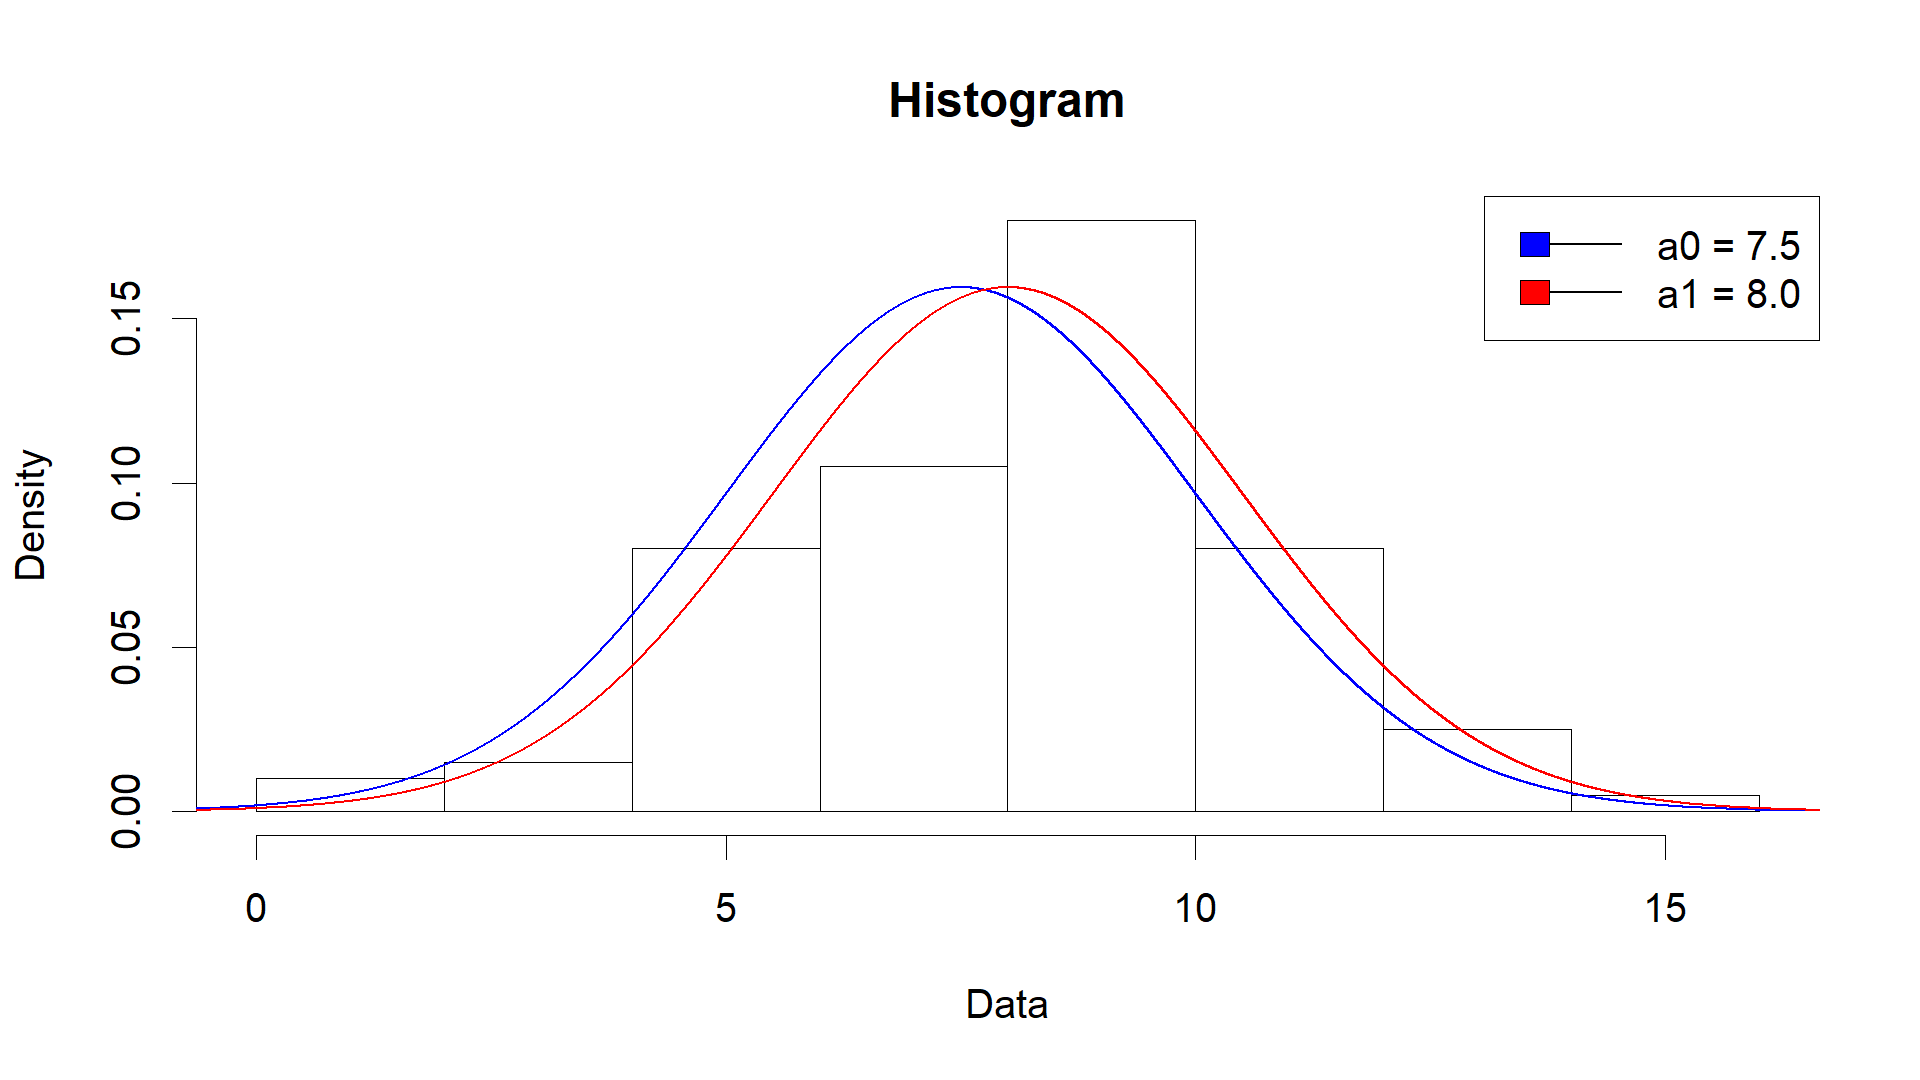
\includegraphics[width=1\linewidth]{../img/hist_densts.png}}
	\caption{Гистограмма частот и графики плотностей.}
	\label{ris:hist_densts}
\end{figure}

По графику видно, что кривая плотности нормального закона для альтернативы $H_1$ ($a=a_1=8.0$) лучше ложится на гистограмму, чем в случае основной гипотезы $H_0$ ($a=a_2=7.5$), что согласуется с выводом в пункте 3.

\end{document}